%\chapterauthor{Author Name}{Author Affiliation}
%\chapterauthor{Second Author}{Second Author Affiliation}
\chapter{Virtualization and Containerization}

One of the major differences between a server and a personal computer is that the server is usually shared among multiple users at the same time. Though working on the same physical server, a user would usually want a private working environment in the server not interrupted by other users. In other words, each and every user would want to ``virtually'' work on an independent and separated computer with his own CPU, RAM, I/O, OS, drives and hard disk storage, despite that the actual hardware is shared with others. This is done through \textit{Virtualization}, which enables running multiple operating systems on a single physical server in an uninterrupted and logically separated manner. The virtually independent computer of such kind is often called a \textit{virtual machine} (VM).

Deploying a new VM would generally consume considerably large amount of time and computational load, because it needs to load the OS in its first startup. Consider a case where there are hundreds of applications, each requiring running in a similar but separate environment. Launching a VM for each application can be a solution, but it can be expensive due to the time and computational burden. It would be batter to rather deploy only one VM (or physical server) with one OS, and put each application in a ``container'' with its own customized drives and configurations. A container is similar with a VM in the sense that it runs separately from other containers. However, a container is much ``lighter'' than a VM, thus is cheaper to launch and manage. This becomes possible thanks to \textit{containerization}. It is worth mentioning that since a container contains all the configuration and minimum requirement information of the application, running a container on different platforms would generate the same stable result. This is handy when comes to code transferring and cross-platform testing.

The similarity and differences of personal PC, VM, and container applications are summarized in Fig. \ref{ch:vac:fig:pcvmcontainersructure}.

\begin{figure}
	\centering
	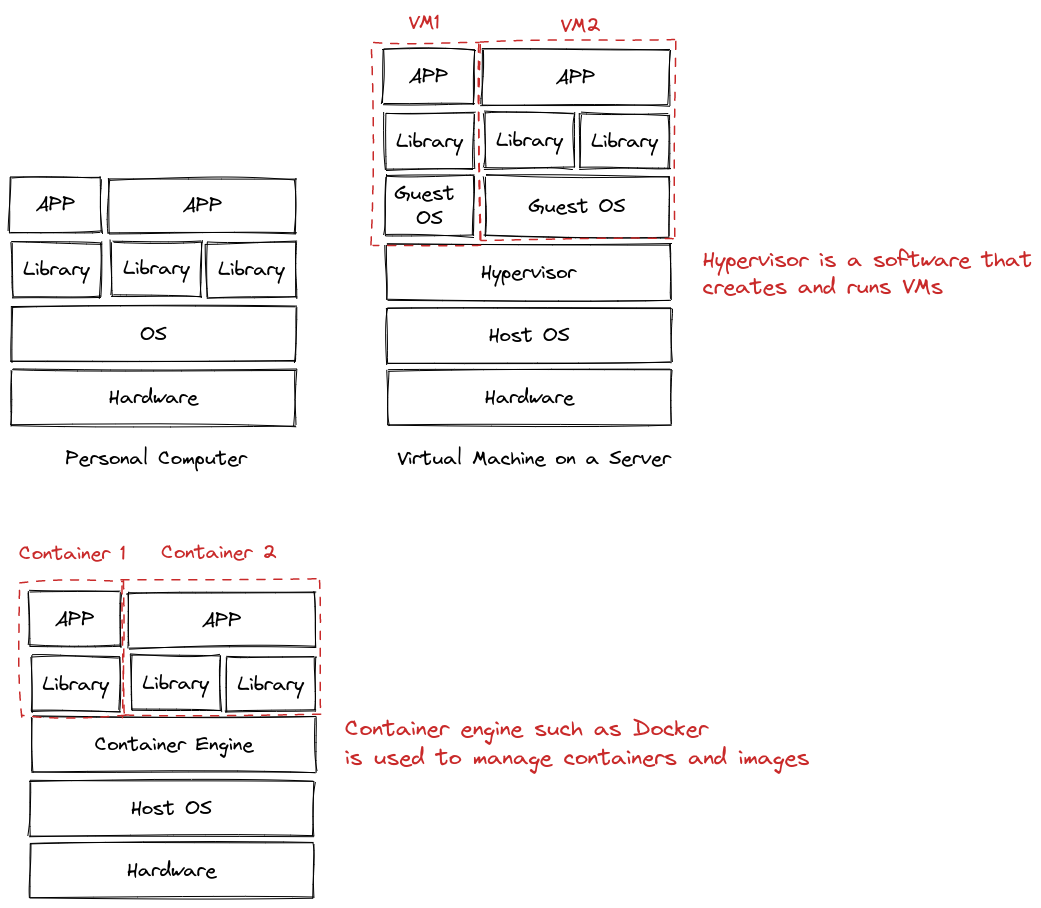
\includegraphics[width=250pt]{chapters/ch_virtualization_and_containerization/figures/pcvmcontainerstructure.png}
	\caption{System architectures of PC, VM and container.} \label{ch:vac:fig:pcvmcontainersructure}
\end{figure}

An an analogy, think of running an APP as asking a restaurant to prepare a dish. The hardware is corresponding with kitchen (along with the cooktop, the frying pan, etc.) of the restaurant where every cooking procedure actually happens. The OS is corresponding with the cook, who uses the materials in the kitchen to make the dish. The OS needs associated drivers and libraries to run the APP correctly. The drivers and libraries are like the skill set expected from the cook in order to prepare the dish correctly. Therefore, installing and configuring drivers and libraries in the OS is like teaching the cook new skills (probably from a cookbook) so that he would know how to cook the dish. Finally, the APP is corresponding with the prepared dish.

In a traditional PC implementation, for each customer (user) or dish (APP), a new kitchen is constructed and its associated cook is hired. The cook is trained to master all necessary skills required by the customer or for the dish. A metaphor of the PC implementation is given in Fig. \ref{ch:vac:fig:acookinakitchen}.
\begin{figure}
	\centering
	
\includegraphics[width=200pt]{chapters/ch_virtualization_and_containerization/figures/acookinakitchen.png}
	\caption{PC implementation: a cook in a kitchen.} \label{ch:vac:fig:acookinakitchen}
\end{figure}

In a VM implementation, a larger and more capable kitchen is setup in advance. For each customer or a dish, a cook is hired. Each cook is trained with the skills necessary for his associated customer or dish. All cooks share the same kitchen. This implementation is more efficient than the previous ``a cook in a kitchen'' implementation in Fig. \ref{ch:vac:fig:acookinakitchen}, as there is no need to scale up the kitchen for each new customer or APP. By sharing the resources among the cooks, it is more probable that the resources in the kitchen be used more effectively. A metaphor of the VM implementation is given in Fig. \ref{ch:vac:fig:manycooksinakitchen}. This is indeed a popular implementation when comes to both enterprise-level server management and a local restaurant.
\begin{figure}
	\centering
	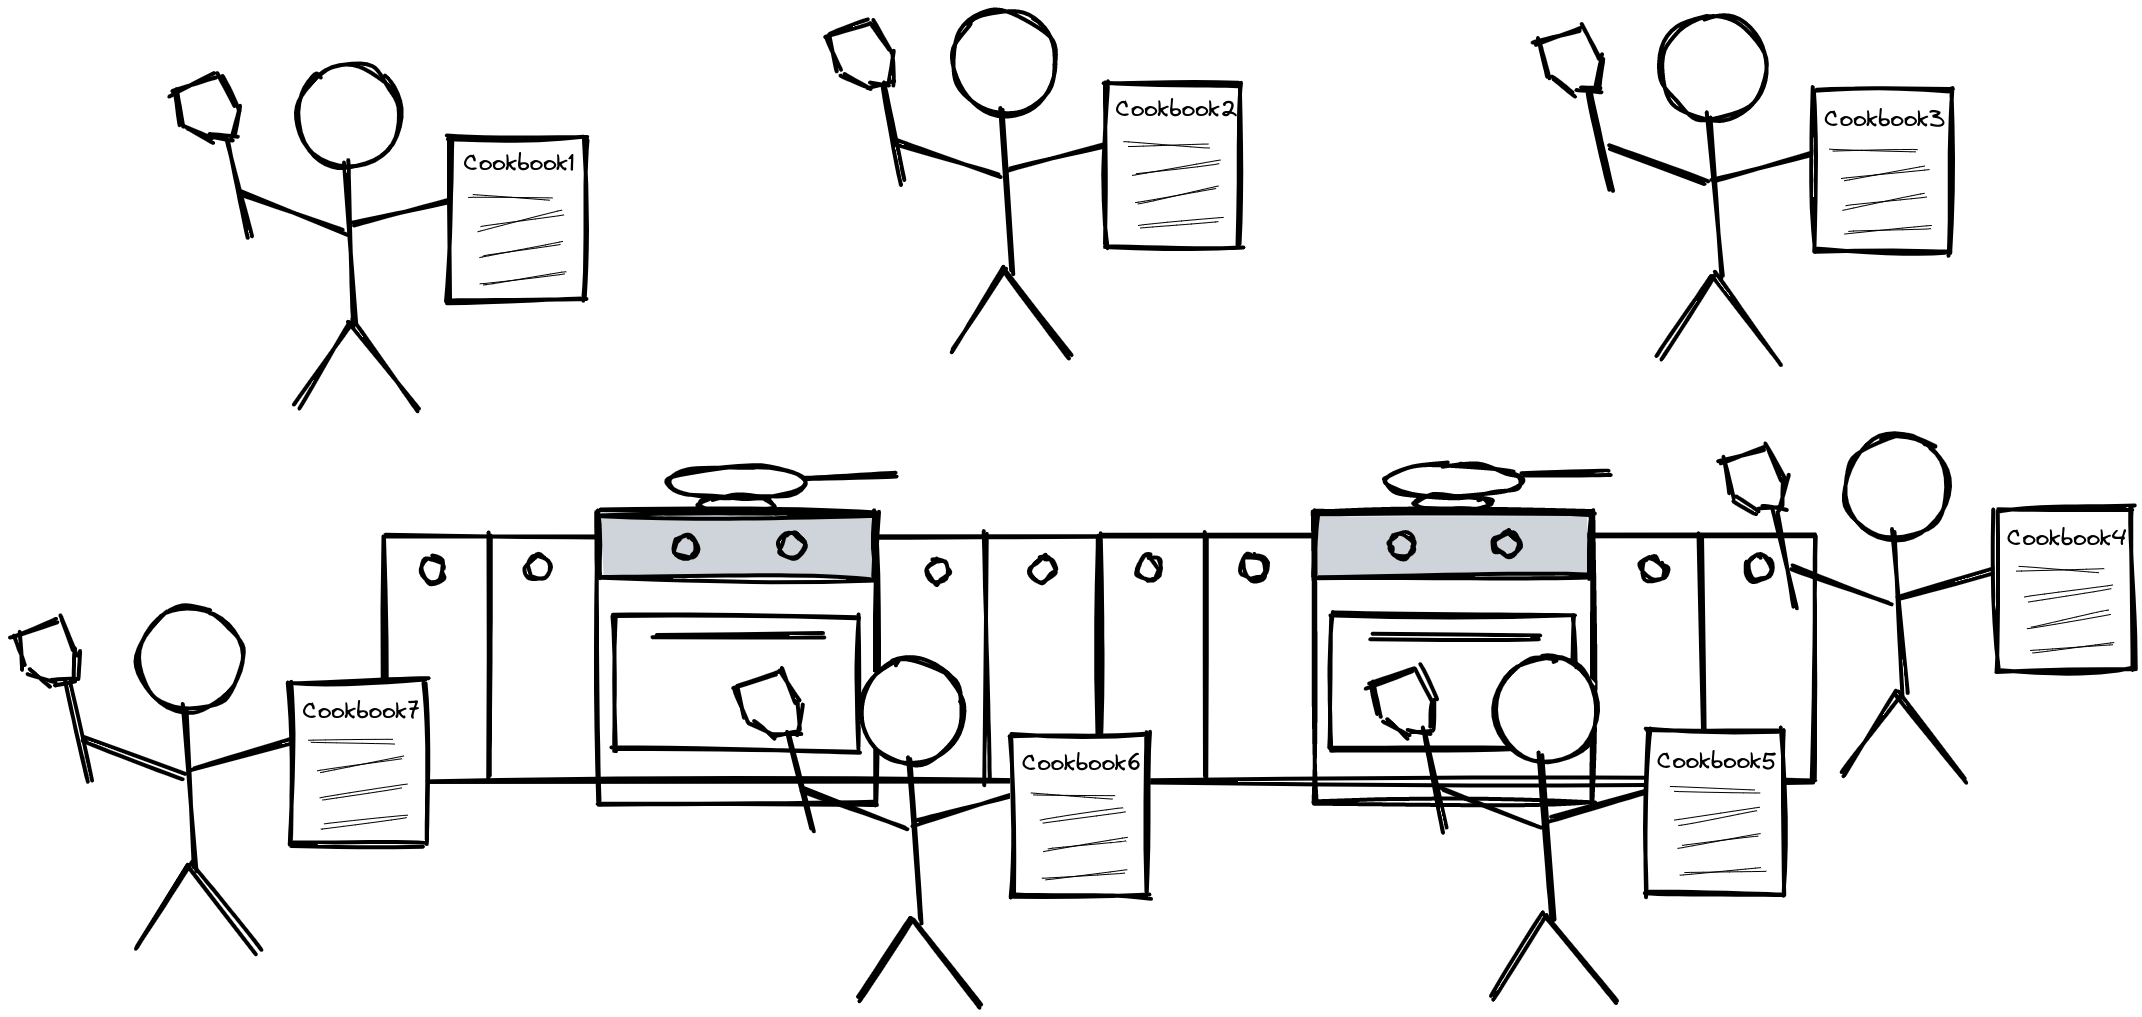
\includegraphics[width=350pt]{chapters/ch_virtualization_and_containerization/figures/manycooksinakitchen.png}
	\caption{VM implementation: many cooks in a kitchen, each with a different cookbook.} \label{ch:vac:fig:manycooksinakitchen}
\end{figure}

Deploy dedicated OS for each APP can be time consuming when the number of the APPs is large. This is also true in the restaurant, where it is very rare for each dish to have a dedicated cook. Instead, a cook usually handles a category of dishes that requires similar skill sets. A cook good at multi-task can handle many dishes by himself alone, as long as the dish recipes are provided. Of course, each dish will stay in its own frypan so that they would not affect each other. This is similar with a container implementation. The recipe for a dish, which describes the skill set of the dish, is called an ``image'' of the container that describes the drivers, libraries and basic configurations for the APP to run. The food cooked in the frypan is the APP. The frypan, the food, and the recipe, together form an instance of a container. A metaphor of the container implementation is given in Fig. \ref{ch:vac:fig:multitaskcook}. Luckily, the cook (OS) is good at multi-tasking by nature, and with the help of a front desk manager (container management tool such as Docker), he can perform quite well.
\begin{figure}
	\centering
	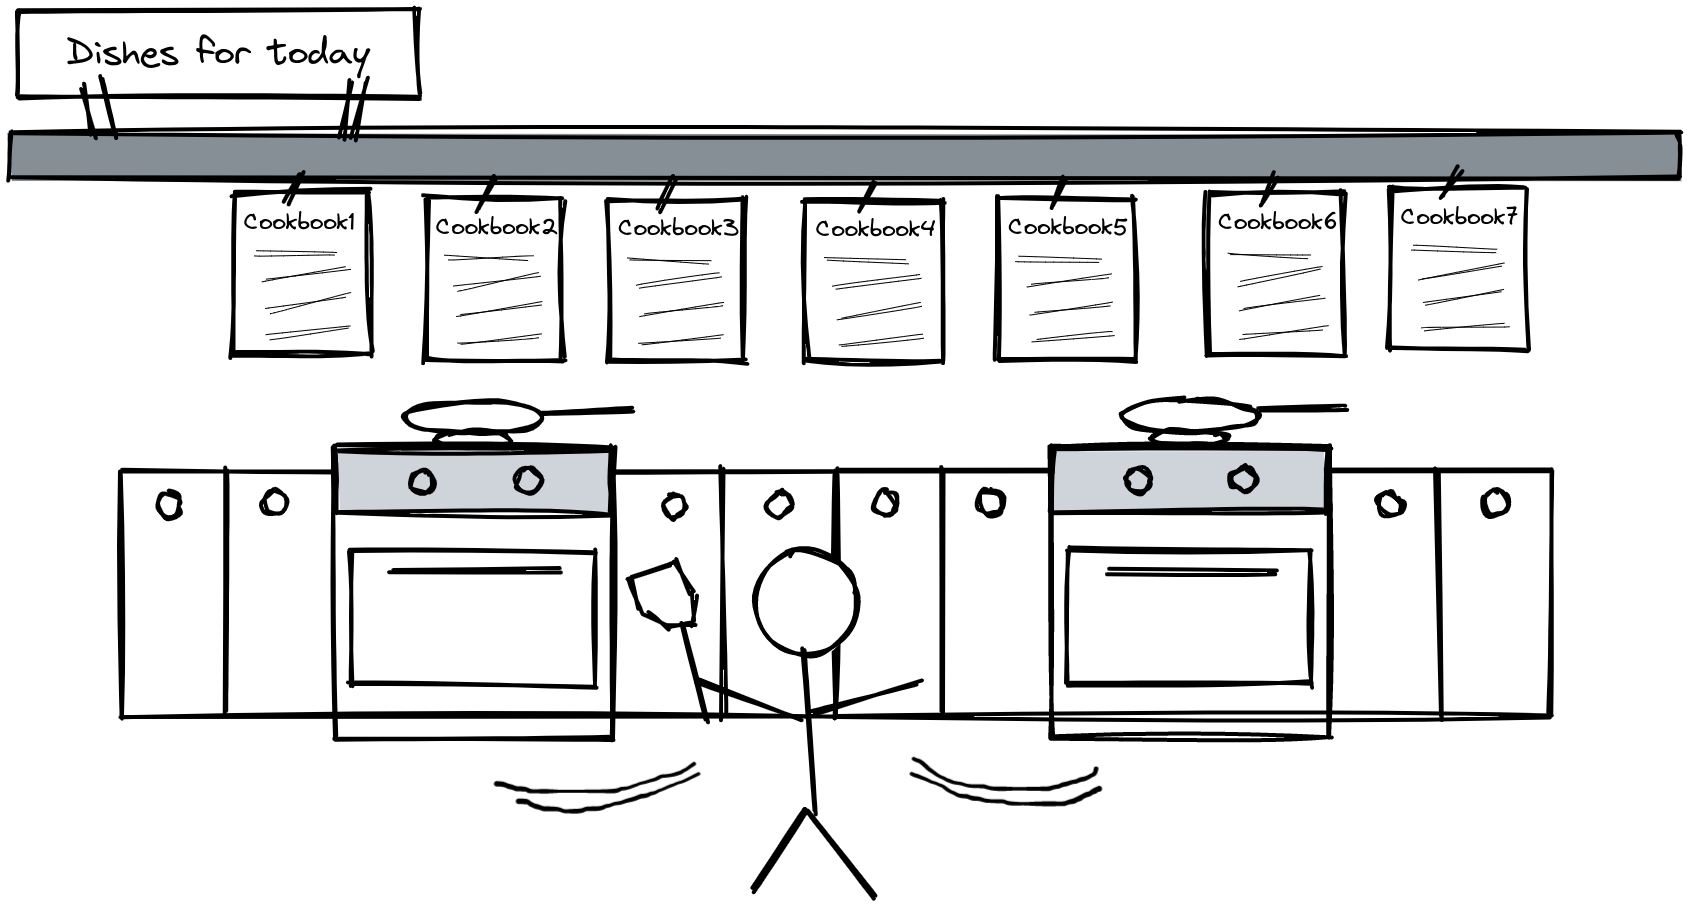
\includegraphics[width=350pt]{chapters/ch_virtualization_and_containerization/figures/multitaskcook.png}
	\caption{Container implementation: one in a kitchen, handling multiple dishes, each has a cookbook and stays in its own pan.} \label{ch:vac:fig:multitaskcook}
\end{figure}

A cookbook is a instruction of a dish. It guarantees that the same dish, even one day to be cooked in a different restaurant by a different cook, would taste the same. Similarly, the image of a container serves as the start-up instruction of the container, and it helps to maintain consistency of the performance of the APP even running on different machines between developers and machines, guaranteeing that a APP runs correctly on different machines. With an image, it is convenient to deploy similar container instances quickly.

\section{Virtual Machine}
...
\section{Container}
...
\section{Docker Basics} \label{ch:vac:sec:db}

Docker and docker hub are widely used container management engine and a platform for sharing container images, respectively. The basic operations of docker engine, including installation of docker engine, using docker engine to run and manage containers, etc., are introduced in this section.

\subsection{Docker Installation}

Docker engine is one of the most popular container management engine available online, and it is free of charge for personal non-commercial usage. To install Docker on a Linux machine, go to \textit{https://www.docker.com/} to for the instruction.

As an example, consider installing Docker engine on Ubuntu. Some of the key steps are summarized as follows.

\vspace{0.1in}
\noindent \textbf{Remove existing Docker engine, if any.}
\begin{lstlisting}
$ sudo apt-get remove docker docker-engine docker.io
$ sudo apt-get remove containerd runc
\end{lstlisting}

\vspace{0.1in}
\noindent \textbf{Add Docker's official GPG key and set up the repository.}
\begin{lstlisting}
$ sudo apt-get update
$ sudo apt-get install ca-certificates curl gnupg lsb-release
$ sudo mkdir -p /etc/apt/keyrings
$ curl -fsSL https://download.docker.com/linux/ubuntu/gpg | sudo gpg --dearmor -o /etc/apt/keyrings/docker.gpg
$ echo \
  "deb [arch=$(dpkg --print-architecture) signed-by=/etc/apt/keyrings/docker.gpg] https://download.docker.com/linux/ubuntu \
  $(lsb_release -cs) stable" | sudo tee /etc/apt/sources.list.d/docker.list > /dev/null
\end{lstlisting}

\vspace{0.1in}
\noindent \textbf{Install Docker.}
\begin{lstlisting}
$ sudo apt-get update
$ sudo apt-get install docker-ce docker-ce-cli containerd.io docker-compose-plugin
\end{lstlisting}

To test whether docker is installed correctly, run
\begin{lstlisting}
$ sudo docker run hello-world
\end{lstlisting}
and if everything is done correctly, a message started with ``Hello from Docker!'' will be displayed in the console, together with a brief introduction to how docker works.

Notice that to use docker commands, sudo privilege is required. To avoid typing \verb|sudo| each time running a docker command, add the user to the docker group as follows.
\begin{lstlisting}
$ sudo usermod <user_name> -aG docker
\end{lstlisting}

In the rest of the section, \verb|sudo| is neglected for docker commands.

\subsection{Launch a Container}

To run a container from an image, simply use
\begin{lstlisting}
$ docker run [image_name]
\end{lstlisting}
Docker will search the local and remote repository for the image, download the image if necessary, and run the container of that image. By default, after successful execution, the container will go into ``Exited'' status. To customize the container running, for example, assigning a name for the container, flags can be used. Details are introduced later.

To check images stored locally, use
\begin{lstlisting}
$ docker image ls
\end{lstlisting}

To check the status of a container, use
\begin{lstlisting}
$ docker container ls
\end{lstlisting}
or
\begin{lstlisting}
$ docker container ls -a
\end{lstlisting}
where \verb|-a| indicates displaying both running and exited containers. Without \verb|-a|, exited containers will not be displayed.

For example, consider running a container of \textit{alpine} as follows. A screen shot is given in Fig. \ref{ch:vac:fig:dockerrunexp}.
\begin{lstlisting}
$ docker run -it --name test-alpine alpine
\end{lstlisting}
where \verb|-i| stands for interactive, which will keep the container's standard input (i.e., the console in this example) open so that the user can actively interract with the container. Option \verb|-t| allocates a pseudo-TTY to the container, making the interactive interface a bit more user friendly. Finally, \verb|--name| assign a name to the container. Without an assigned name, docker will randomly assign a name to the container.
\begin{figure}
	\centering
	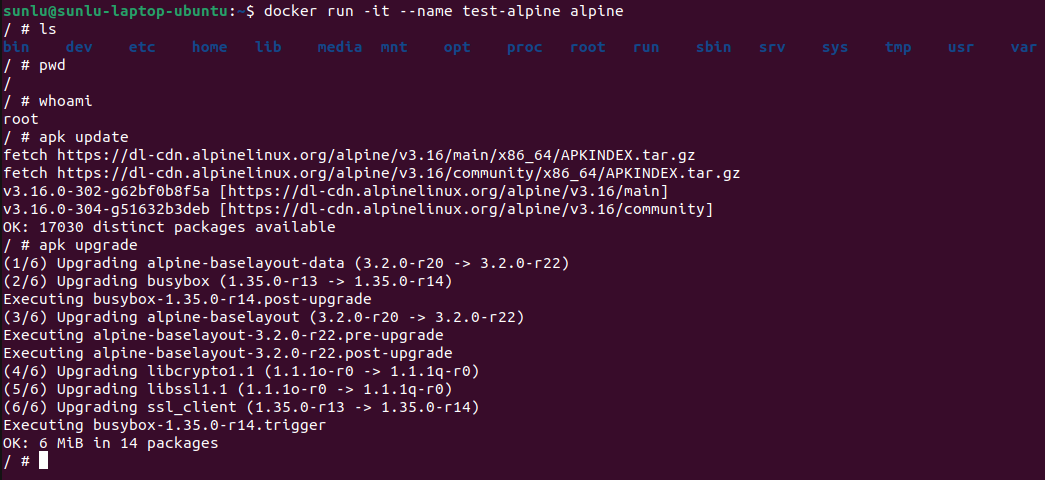
\includegraphics[width=350pt]{chapters/ch_virtualization_and_containerization/figures/dockerrunexp.png}
	\caption{An example of running \textit{apline} container, with interactive TTY and name \textit{test-apline}.} \label{ch:vac:fig:dockerrunexp}
\end{figure}

It can be seen from Fig. \ref{ch:vac:fig:dockerrunexp} that once the container is started, the user can interact with the container using its shell, and perform actions such as upgrading the container, or deploy a web server, etc. While keep the container up running, open another terminal and use \verb|docker container ls|. The container \verb|test-alpine| shall appear in the list, as shown in Fig. \ref{ch:vac:fig:dockerrunexppart2}.
\begin{figure}
	\centering
	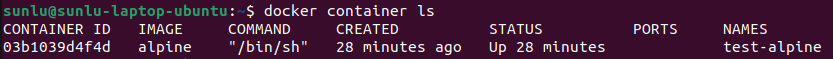
\includegraphics[width=250pt]{chapters/ch_virtualization_and_containerization/figures/dockerrunexppart2.png}
	\caption{List the up running container \textit{test-apline}.} \label{ch:vac:fig:dockerrunexppart2}
\end{figure}

If exit from Fig. \ref{ch:vac:fig:dockerrunexp} (by using \verb|exit| in the container), the container will transfer its status from up running to exited, as shown in Fig. \ref{ch:vac:fig:dockerrunexppart3}.
\begin{figure}
	\centering
	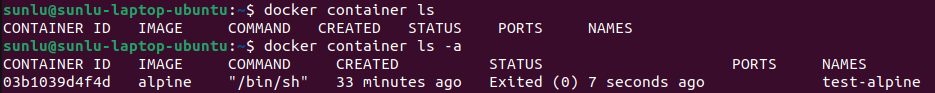
\includegraphics[width=250pt]{chapters/ch_virtualization_and_containerization/figures/dockerrunexppart3.png}
	\caption{List the exited container \textit{test-apline}.} \label{ch:vac:fig:dockerrunexppart3}
\end{figure}

It is also possible to launch a container and let it run in the background using \verb|-d| flag. An example is given below.
\begin{lstlisting}
$ docker run -dt --name test-background-alpine alpine
\end{lstlisting}
By changing \verb|-i| to \verb|-d|, the container runs in the background without accessing its interactive shell interface. The status of the container, after executing the above command, will stary up running and can be listed by \verb|docker container ls|.

In summary, selected key commands regarding launching a container is given in Table \ref{ch:vac:tab:launchcontainer}.

\begin{table}
	\centering \caption{Commonly used docker commands to launch a container.}\label{ch:vac:tab:launchcontainer}
	\begin{tabularx}{\textwidth}{llX}
		\hline
		Command & Flag & Description \\ \hline
		\verb|docker run| & --- & Launch a container of the image followed by the command. If the image cannot be found locally, it downloads the image from the remote repository automatically. Assign a random name to the container. Exit the container after execution. \\ \hdashline
        \verb|docker run| & \verb|-i| & Keep the standard input of the container open when launching the container. \\ \hdashline
        \verb|docker run| & \verb|-d| & Launch the container in the background and keep it up running. \\ \hdashline
        \verb|docker run| & \verb|-rm| & Automatically remove the container when exiting. The removed container will not be listed in \verb|docker container ls -a|. This is usually used for testing and debugging. \\ \hdashline
        \verb|docker run| & \verb|-t| & Allocate a pseudo-TTY. TTY stands for ``TeleTYpewriter''. A simplified explanation to \verb|-t| is that it makes sure that the I/O of the container follows the typical terminal format. The flag usually comes with the flags \verb|-i| or \verb|-d|, to form \verb|-it| or \verb|-dt|. \\ \hdashline
        \verb|docker run| & \verb|--restart| & Indicates in which condition the container needs to restart. This is usually used on containers running in the background, i.e., it usually comes with the flag \verb|-dt|. Commonly used restart configurations include \verb|--restart no| (do not automatically restart container when it exits), \verb|--restart on-failure[:max_retries]| (restart if the container exits with a non-zero exit status), \verb|--restart always| (restart regardless of the exit status). Notice that for a container with \verb|--restart| flag, it is still possible to stop and remove the container manually. \\ \hdashline
        \verb|docker run| & \verb|--name| & Assign a name to the container. \\ \hline
        \verb|docker image ls| & --- & List local images. \\ \hline
        \verb|docker container ls| & --- & List up running containers. \\ \hdashline
        \verb|docker container ls| & \verb|-a| & List all containers. \\
		\hline
	\end{tabularx}
\end{table}

\subsection{Access and Manage a Container}

To start an existing (but exited) container, use
\begin{lstlisting}
$ docker start <container_name>
\end{lstlisting}
This command starts the exited container, and keep it up running in the background.

For a container running in the background, use \verb|docker exec| to execute a shell command as follows.
\begin{lstlisting}
$ docker exec <container_name> <command>
\end{lstlisting}

To enable the TTY shell of a container running in the background, use
\begin{lstlisting}
$ docker exec -it <container_name> <shell_name>
\end{lstlisting}
where depending on the environment of the container, the shell can be different. In the case of an \textit{alpine} imgae based container, \verb|ash| is the default shell. For a \textit{ubuntu} image based container, on the other hand, usually \verb|bash| should be specified.

There are multiple ways and protocols to interact with the file systems in a container, depending the I/O setup of the container. For a container running locally, \verb|docker cp| can be conveniently used for file transfer between the container and the host machine as follows. From container to host machine:
\begin{lstlisting}
$ docker cp <container_name>:<source> <destination>
\end{lstlisting}
and from host machine to container:
\begin{lstlisting}
$ docker cp <source> <container_name>:<destination>
\end{lstlisting}
where \verb|[source]| and \verb|[destination]| refer to the path to the source and destination, respectively, located in the host machine or the container.

To stop or restart a container running in the background, use
\begin{lstlisting}
$ docker stop <container_name>
$ docker restart <container_name>
\end{lstlisting}
respectively. When a container is stopped, it enters exited status.

To remove a stopped container, use
\begin{lstlisting}
$ docker container rm <container_name>
\end{lstlisting}
to remove a specific container, or
\begin{lstlisting}
$ docker container prune
\end{lstlisting}
to remove all stopped containers.

To rename a container (without changing its container ID or anything else), use
\begin{lstlisting}
$ docker rename <old_container_name> <new_container_name>
\end{lstlisting}

To quickly check container status (CPU, memory usage, etc.) of an up running container or all up running containers, use
\begin{lstlisting}
$ docker stats <container_name>
\end{lstlisting}
where the container name can be specified as an option.

To list down more detailed information of a container, including its status, gateway, IP address, etc., use
\begin{lstlisting}
$ docker inspect <container_name>
\end{lstlisting}

To create an image from a container, use
\begin{lstlisting}
$ docker commit <container_name> <image_name>
\end{lstlisting}
The \verb|docker commit| command saves the container's file changes or settings into a new image, which allows easier populating containers or debugging in a later stage. Notice that \verb|docker commit| does not save everything of the container into the image.

\subsection{Publish a Container}

A container can be configured to be accessible from not only the host machine but also other computers from outside the world. In a typical web service application, the host machine and the containers are often designed following the architecture similar with Fig. \ref{ch:vac:fig:containerwebserverarchitecture}. The containers shall be configured similarly to provide consistent services. A web server, such as \textit{apache} or \textit{nginx}, shall be installed and kept running in the containers. The load balancer is a special software toolkit that monitor the status of the containers, manage the dataflow, and scale up and down the number of containers depending on the total service requests.
\begin{figure}
	\centering
	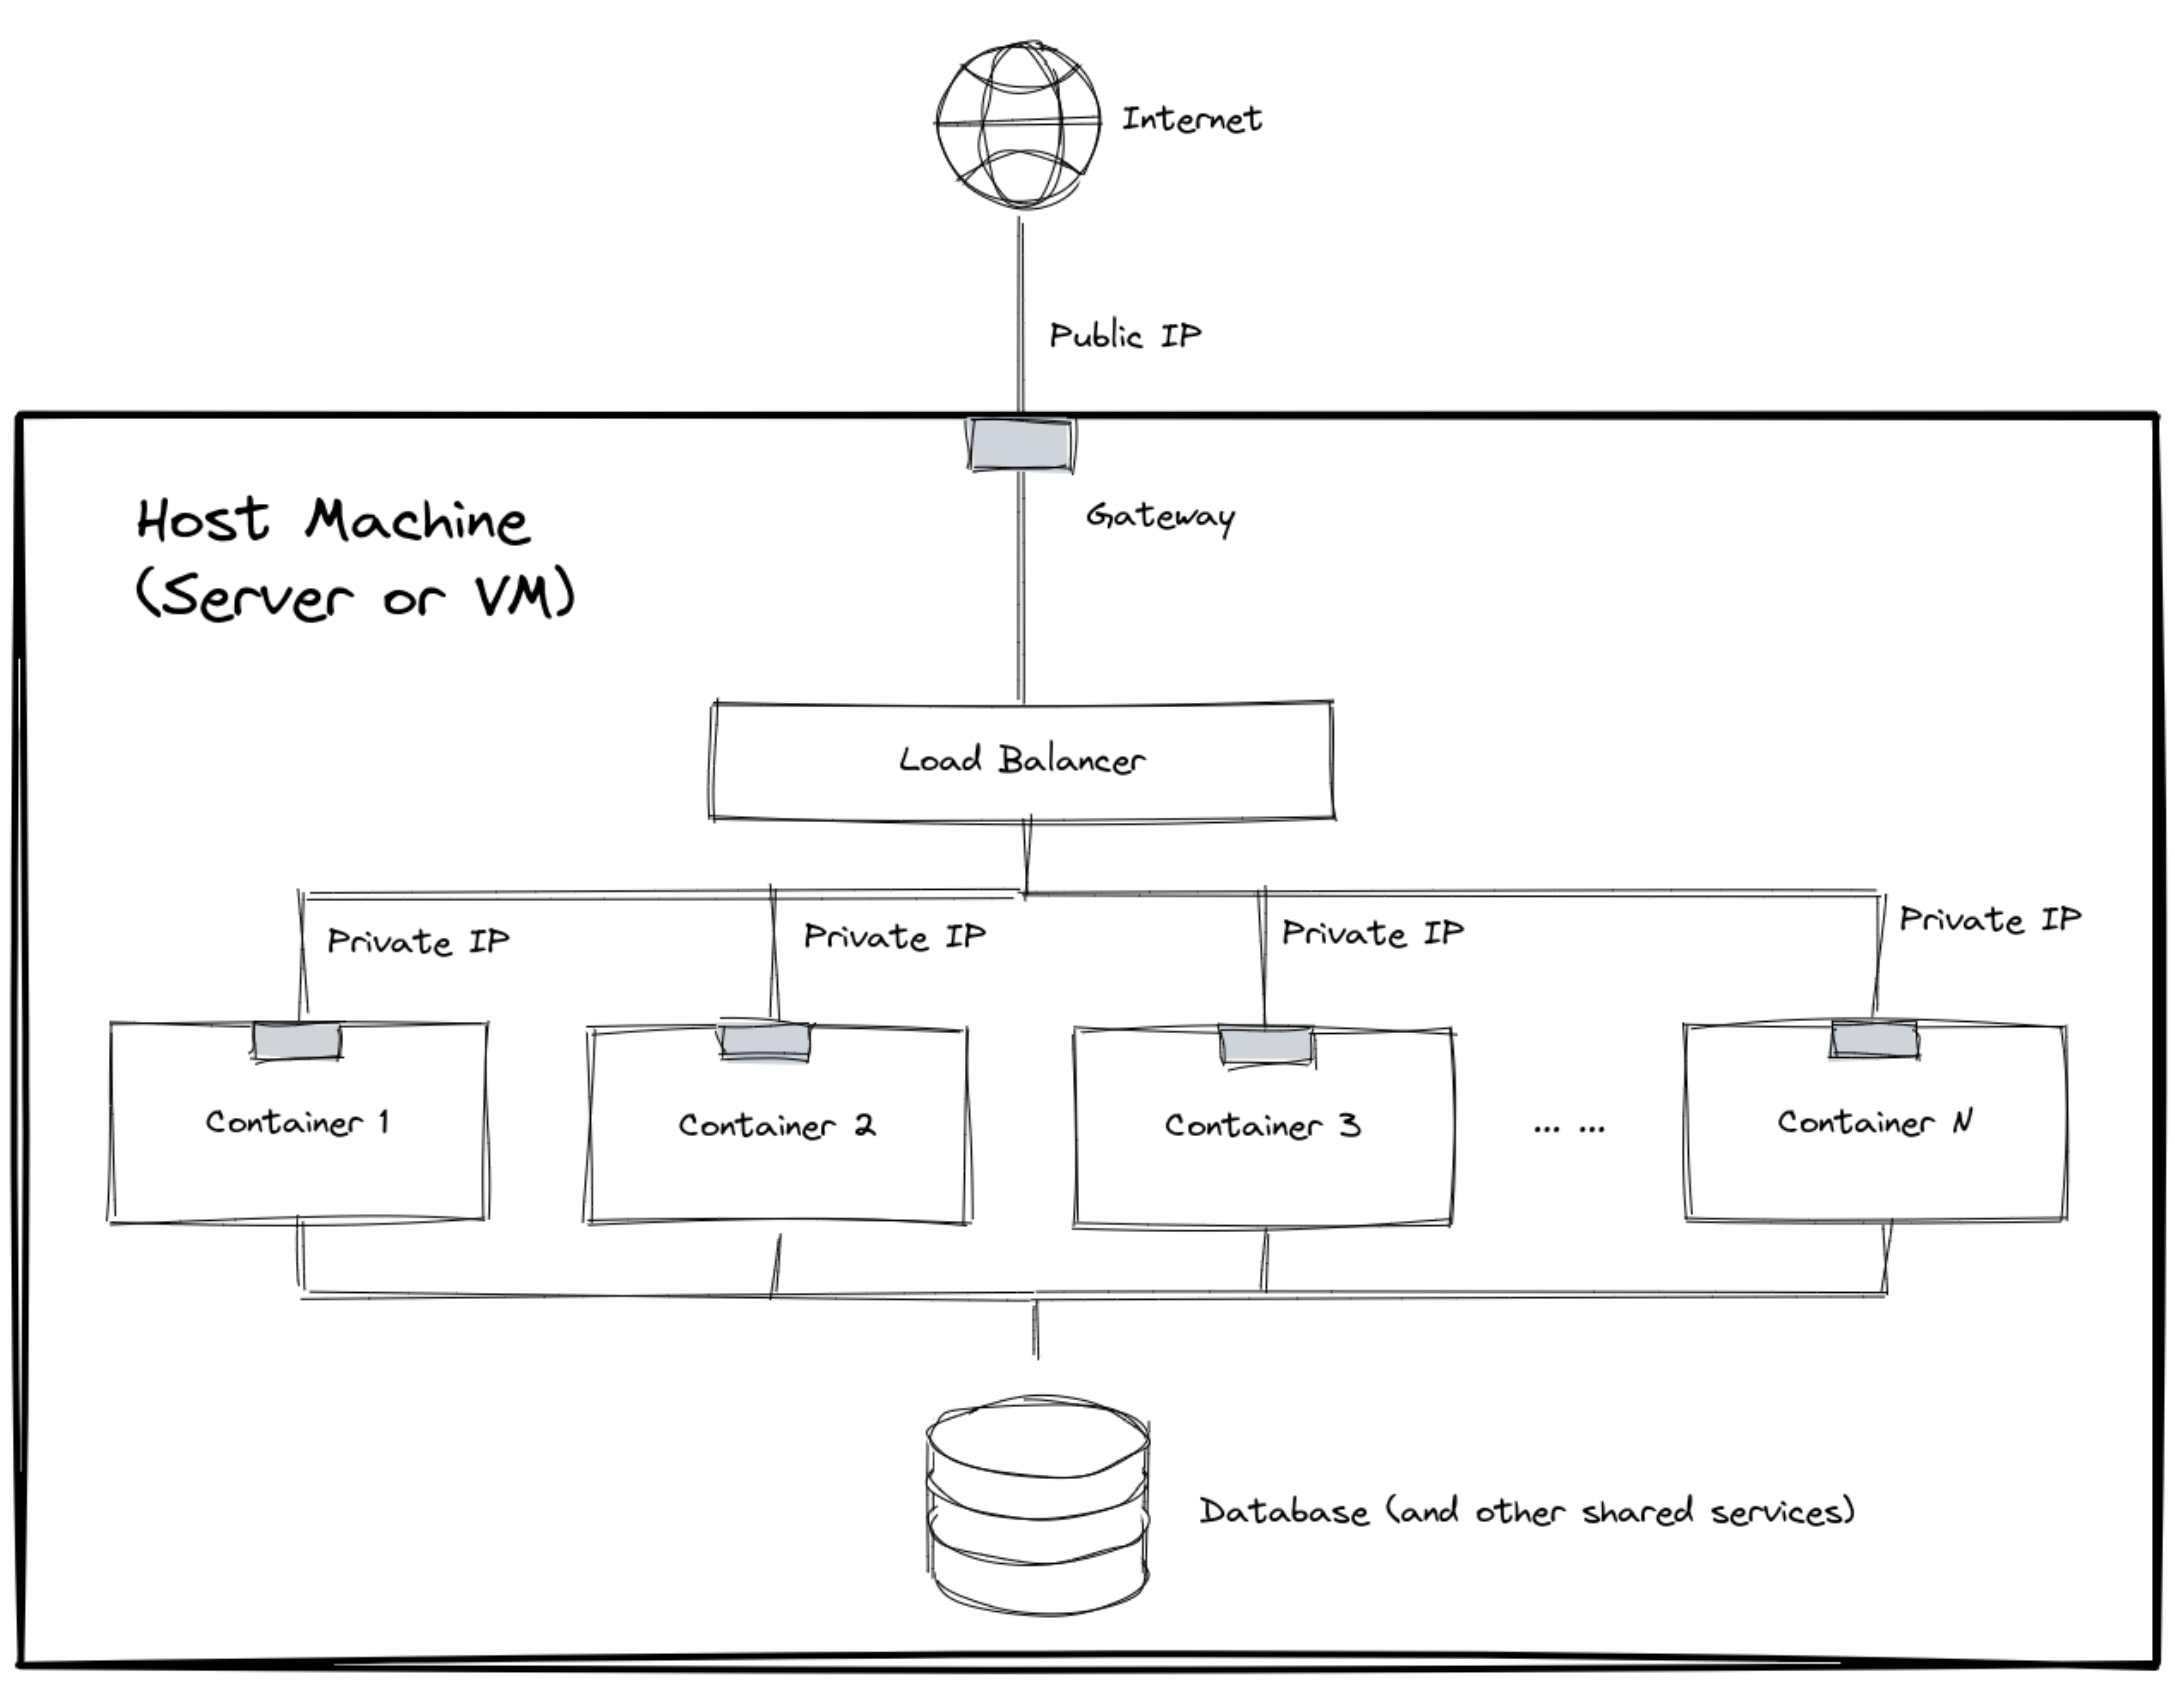
\includegraphics[width=350pt]{chapters/ch_virtualization_and_containerization/figures/containerwebserverarchitecture.png}
	\caption{A simplified architecture where containers are used to host the web service.} \label{ch:vac:fig:containerwebserverarchitecture}
\end{figure}

An example of setting up a web server in containers from scratch is given in this section. For simplicity, only one container is used and the load balancer and the shared services are not included in the example.

As a first step, create a container from the official \textit{nginx} image as follows. Notice that it is also possible to create containers from \textit{apline}, and install \textit{nginx} on the container.
\begin{lstlisting}
$ docker run -dt --name simple-web nginx
\end{lstlisting}

The second step is to create configuration file for \textit{nginx}, and also the \textit{html} files to used as the static web page. For convenience, the files are created and edited in the host machine, then copied to the container. The following \textit{default.conf} and \textit{index.html} have been created, respectively. The configuration file \textit{default.conf}:
\begin{lstlisting}
server {
	listen 80 default_server;
	listen [::]:80 default_server;
	root /var/www/html/;
}
\end{lstlisting}
and the \textit{html} file \textit{index.html}:
\begin{lstlisting}
<html>
	<body>
		<h1>Hello World!</h1>
	</body>
</html>
\end{lstlisting}

Use \verb|docker copy| to copy the two files to the designed locations in the container as follows.
\begin{lstlisting}
$ docker exec simple-web mkdir /var/www
$ docker exec simple-web mkdir /var/www/html
$ docker cp default.conf simple-web:/etc/nginx/conf.d/default.conf
$ docker cp index.html simple-web:/var/www/html/index.html
\end{lstlisting}

Change the ownership of the \textit{html} file as follows, so that the current user \textit{nginx} is able to access that file.
\begin{lstlisting}
docker exec simple-web chown -R nginx:nginx /var/www/html
\end{lstlisting}

Reload and configuration file and restart the web server as follows.
\begin{lstlisting}
docker exec simple-web nginx -s reload
\end{lstlisting}

To test the web server running inside the container, obtain the IP address of the container using
\begin{lstlisting}
$ docker inspect simple-web | grep IPAddress
\end{lstlisting}
and open a browser with the obtained IP address keyed in. By default, the browser would try to access port 80 of the container, and the ``Hello World!'' web page shall show up.

The last step is to commit the container into a new image using \verb|docker commit|, and subsequently populate the containers as follows.
\begin{lstlisting}
$ docker commit simple-web simple-web-image
$ docker run -dt --name web01 -p 80:80 simple-web-image
\end{lstlisting}

Notice that different from the previous container ``\textit{simple-web}'', the new container ``\textit{web01}'' IP address port 80 is mapped with the port 80 of the host machine. Therefore, the web page hosted in ``\textit{web01}'' can be accessed not only by the container's IP address, but also by the host machine IP address. Key in \verb|localhost| in the browser on the host machine and the ``Hello World!'' web page shall show up.

\section{Docker Images}

In earlier Section \ref{ch:vac:sec:db}, images have been used to create containers. An image performs like a template or source of a container. It contains the basic settings, initial configurations, required libraries, and other metadata of the container. Every image comes with a ``step-by-step guidance'' to set up the container, known as the \textit{Dockerfile}. More details about the formulation and function of a docker image are introduced in the rest of this section.

\subsection{Image Architecture}

An image shall contain everything needed to create and initialize a container. This include but not limited to:
\begin{itemize}
  \item A ``step-by-step guidance'' of all procedures to create the container, i.e., the \textit{Dockerfile}.
  \item Filesystem architecture of the container.
  \item All libraries and driver software to be installed in the container upon creation.
  \item Necessary code for initialization.
\end{itemize} 
In addition, an image shall be designed and organized in such a way that it is migratable, reusable and light, and can be used to easily populate large number of containers. For better inheritability, an image might be based on another existing image, which is called its parent image. An image with no parent, such as the official \textit{hello-world} image from Docker Hub, is called a base image.

\subsection{Dockerfile}

Dockerfile is a human-readable text document that serves as an instruction for building an image. As mentioned earlier, a Dockerfile is essentially a step-by-step guidance to create a container associated with the image. Like other computer languages, Dockerfile has reserved keywords, environmental variables, syntax and grammar rules. Only the basics of forming a Dockerfile is introduced in this section. More details can be found in the docker reference from the official website.

Just as a quick example, the Dockerfile of the official \textit{hello-world} image from Docker Hub look like the following.
\begin{lstlisting}
FROM scratch
COPY hello /
CMD ["/hello"]
\end{lstlisting}
where \verb|FROM scratch| indicates that this image is a base image without a parent. The following \verb|COPY hello /| basically copies the \textit{hello} binary script in the image to the root of the container. Finally, \verb|CMD ["/hello"]| executes \textit{hello} binary script and print the welcome messages in the console.

Intuitively, a typical Dockerfile shall at the minimum include following steps:
\begin{enumerate}[(1)]
  \item Define parent image using \verb|FROM|.
  \item Create filesystem architecture of the container, and correct the ownership of files in the file system using \verb|RUN|.
  \item Set working directory using \verb|WORKDIR|.
  \item Copy files to the container using \verb|COPY| or \verb|ADD|.
  \item Configure registry using \verb|RUN|.
  \item Install packages from the registry using \verb|RUN|.
  \item Copy more files to the container using \verb|COPY| or \verb|ADD|.
  \item Switch to the node user using \verb|USER|.
  \item Expose port using \verb|EXPORT|.
  \item Run the APP using \verb|CMD|.
\end{enumerate}

\subsection{Basic Docker Image Operations}

...

\subsection{Image Sharing on Docker Hub}


...
















